\setchapterpreamble[u]{\margintoc}
\chapter{Գծային ձևափոխություններ}
\labch{matrices}

\emergencystretch 2em

\section{Գծային տարածություններ}

Դիտարկենք հետևյալ երեք բազմությունները․
\begin{itemize}
    \item թվանշանների $D=\{0, 1, 2, \dots, 9\}$ բազմությունը
    \item դրական թվերի $P=\{x \in \R : x > 0\}$ բազմությունը
    \item երկչափ վեկտորների $\R^2$ բազմությունը
\end{itemize}

Եթե փորձենք վերցնել յուրաքանչյուր բազմությունից երկու տարր և գումարել իրար, ապա ցանկացած երկու դրական թիվ գումարելով՝ կստանանք դրական թիվ, ցանկացած երկու երկչափ վեկտոր գումարելով՝ կստանանք նորից երկչափ վեկտոր, իսկ այ երկու թվանշան գումարելիս հնարավոր է, որ թվանշան չստացվի (օրինակ՝ $5 + 7 = 12$, որը $D$-ից չէ)։ Այս դեպքում ասում են, որ $P$ և $\R^2$ բազմությունները \textit{փակ են գումարման նկատմամբ։}

Նման ձևով, եթե յուրաքանչյուր բազմությունից վերցնենք որևէ տարր ու բազմապատկենք ինչ-որ $c\in \R$ թվով/սկալյարով, ապա հնարավոր է, որ $D$-ի դեպքում՝ ստացվածը չլինի թվանշան (օրինակ՝ $5 \cdot c$, որտեղ $c=1000$), իսկ $P$-ի դեպքում՝ չլինի դրական թիվ (օրինակ՝ $12 \cdot c$, որտեղ $c=-1$): Մյուս կողմից՝ $\R^2$-ից ինչ վեկտոր էլ վերցնենք և ինչ $c$ թվով էլ բազմապատկենք, $\R^2$ բազմությունից դուրս չենք կարող հայտնվել․ միշտ ստանալու ենք ինչ-որ երկչափ վեկտոր $\R^2$-ից։ Ինչպես կռահում եք, $\R^2$-ը կոչվում է \textit{փակ թվով բազմապատկման նկատմամբ} (իսկ $D$-ն ու $P$-ն փակ չեն)։

Գումարման և թվով բազմապատկման նկատմամբ փակ լինելը շատ օգտակար հատկություն է, քանի որ այդ դեպքում առանց բազմությունից դուրս գալու կարելի է բազմության տարրերը ազատորեն գումարել-հանել կամ բազմապատկել թվերով, ու արդյունքում մնալ միևնույն բազմության մեջ։

\begin{figure}[h]
\centering
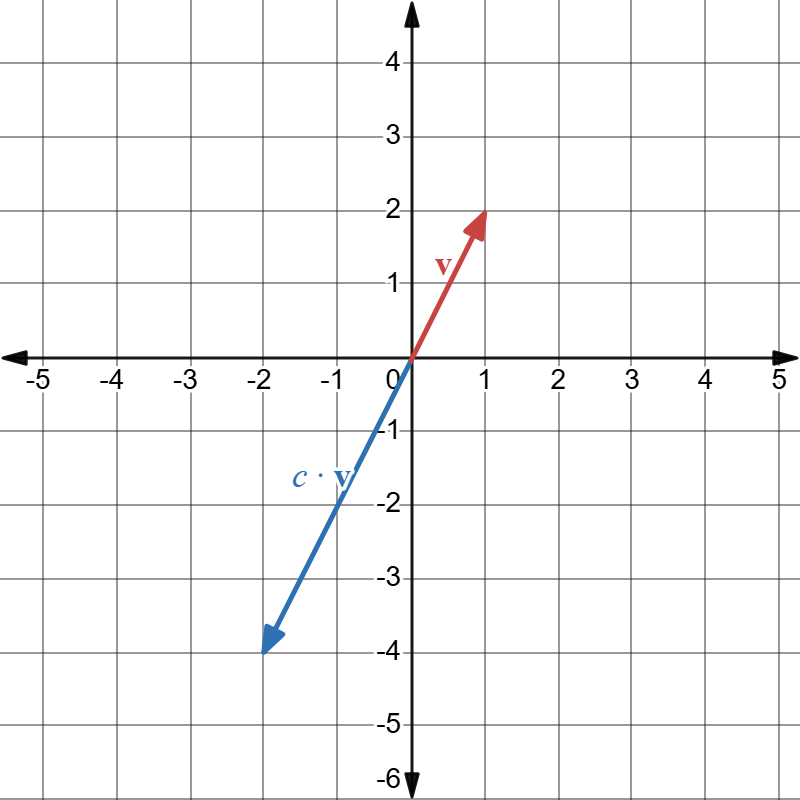
\includegraphics[width=0.5\linewidth]{chapters/chapter 2/y=2x 2.png}
\end{figure}

Պարզվում է՝ միայն $\R^2$-ը չէ, որ օժտված է այդ լավ հատկություններով։ Վերցնենք, օրինակ, $y=2x$ ուղիղը և դրա վրա ընտրենք ցանկացած $\vv$ վեկտոր։ Ինչպիսի $c\in \R$ թվով էլ այն բազմապատկենք, արդյունքում ստացված վեկտորը նորից ընկած է լինելու $y=2x$ ուղղի վրա։ Նույն կերպ, ինչ երկու $\vv_1$, $\vv_2$ վեկտորներ էլ վերցնենք այս ուղղի վրա և գումարենք իրար, ստացվածը կրկին $y=2x$-ի վրա է լինելու։ 

Այլ կերպ ասած՝ ինչպես $\R^2$-ը, այնպես էլ $y=2x$ ուղիղը (գիծը) \textbf{փակ է գումարման և թվով բազմապատկման նկատմամբ։} 

\question{Իսկ ի՞նչ կարող եք ասել $y=2x+1$ ուղղի մասին։}

Նմանատիպ օգտակար բազմությունները, որոնց տարրերը կարելի է ազատորեն
\begin{itemize}
    \item գումարել-հանել
    \item գումարելիների տեղերը փոխել
    \item գումարման ու թվով բազմապատկման հերթականությունը փոխել
    \item փակագծերը բացել
\end{itemize}
և այլն՝ առանց այդ բազմությունից դուրս\marginnote{
$\R^2$-ը գծային տարածություն է, իսկ $y=2x$ ուղիղը նրա ենթատարածություն է} հայտնվելու, կանվանենք \textit{գծային տարածություններ։} 

\begin{definition}
$V$ բազմությունը կոչվում է \textbf{գծային} (կամ վեկտո\-րա\-կան) \textbf{տարածություն,} եթե այն
\begin{enumerate}
\item փակ է գումարման և թվով բազմապատկման\marginnote{ցանկացած իրական թվով} նկատմամբ
\end{enumerate}
և նրա տարրերը բավարարում են հետևյալ հատկություններին․
\begin{enumerate}[resume]
  \item \( (\mathbf{u} + \mathbf{v}) + \mathbf{w} = \mathbf{u} + (\mathbf{v} + \mathbf{w}) \)
  \item \( \mathbf{u} + \mathbf{v} = \mathbf{v} + \mathbf{u} \)
  \item կա մի այնպիսի \( \mathbf{0} \) տարր, որ \( \mathbf{v} + \mathbf{0} = \mathbf{v} \) ցանկացած \( \mathbf{v} \in V \) համար
  \item ցանկացած \( \mathbf{v} \in V \) տարրի համար կա այնպիսի \( \overline{\vv} \) տարր,\marginnote{այսինքն՝ ամեն $\vv$-ի հակադիր ևս $V$-ից է} որ \( \mathbf{v} + \overline{\vv} = \mathbf{0} \)
  \item \( (cd) \cdot \mathbf{v} = c \cdot (d \cdot \mathbf{v}) \)
  \item \( 1 \cdot \mathbf{v} = \mathbf{v} \)
  \item \( c \cdot (\mathbf{u} + \mathbf{v}) = c \cdot \mathbf{u} + c \cdot \mathbf{v} \)
  \item \( (c + d) \cdot \mathbf{v} = c \cdot \mathbf{v} + d \cdot \mathbf{v} \)
\end{enumerate}
\end{definition}

Հատկությունները անգիր անելու կարիք չկա․ դրանք այն բնական հատկություններն են, առանց որոնց կդժվարանայինք աշխատել վեկտորների հետ։


\section{Ենթատարածություններ}


Այսպիսով, $\R^2$-ը ($\R^1$-ը, $\R^3$-ը, ...) գծային տարածություն է։ Բայց նրանում ընկած $y=2x$ ուղիղը նույնպես բավարարում է 1-9 պայման\-նե\-րին, հետևաբար այն նույնպես գծային տարածություն է։ 

\begin{definition}
$V$ գծային տարածության $U$ ենթաբազմությունը կոչվում է $V$-ի \textbf{ենթատարածություն,} եթե այն ինքը գծային տարածություն է։
\end{definition}

\begin{example} 
Գծային տարածություններ են օրինակ՝
\begin{itemize}
\item բոլոր $\R^n$-երը,

\item իրական թվերի $\R$ բազմությունը,

\item $\R^2$ հարթության $(0, 0)$ սկզբնակետով անցնող ցանկացած ուղիղ (հետևաբար դրանք $\R^2$-ի ենթատարածություններ են),

\item $\R^3$ տարածության $(0, 0, 0)$ սկզբնակետով անցնող ցանկացած ուղիղ և ցանկացած հարթություն (հետևաբար դրանք $\R^3$-ի ենթա\-տարածու\-թյուններ են),


\item միայն $\mathbf{0}$-ից բաղկացած $\{\mathbf{0}\}$ բազմությունը,
\end{itemize}
բայց միևնույն ժամանակ՝
\begin{itemize}
\item բնական թվերի բազմությունը,

\item դրական թվերի բազմությունը,

\item $\R^2$-ի՝ $y$-ների առանցքից վերև ընկած վեկտորների բազմությունը
\end{itemize}
գծային տարածություններ չեն։
\end{example}

Իրականում, եթե ունենք ինչ-որ $V$ գծային տարածություն և դրա մի որևէ $U$ ենթաբազմություն,\marginnote{որպես օրինակ՝ պատկերացրեք $V=\R^2$, իսկ $U$-ն $y=2x$ ուղիղն է $\R^2$-ում} ապա դժվար չէ պարզել՝ $U$-ն իրենով գծային (ենթա)տարածություն է, թե ոչ։ Պարզվում է, որ եթե $U$-ն փակ է գումարման և թվով բազմապատկման նկատմամբ, ապա դա \textit{բավարար} է, որ այն լինի $V$-ի ենթատարածություն։ 

\begin{theorem}
Եթե $V$-ն գծային տարածություն է, իսկ $U$-ն նրա որևէ ենթաբազմություն, ապա $U$-ն կլինի $V$-ի ենթատարածություն այն և միայն այն դեպքում, եթե  
\begin{enumerate}
\item $\vx+\vy \in U$ ցանկացած $\vx,\ \vy\in U$ համար,
\item $c\vx \in U$ ցանկացած $\vx\in U$ և $c\in\R$ համար։
\end{enumerate}
\end{theorem}

Այսինքն՝ եթե $U$-ն փակ է գումարման ու թվով բազմապատկման նկատմամբ, ապա մնացած 2-9 օգտակար հատկությունները այն արդեն ժառանգում է $V$-ից (հետևաբար դառնում գծային տարածություն)։

\warning{Թեորեմը աշխատում է, միայն եթե $V$-ն գծային տարածություն է։}



\section{Մատրիցներ}

Այժմ պատրաստվում ենք $\R^n$ տարածությունը պտտել, շրջել, ռեզինի նման ձգել ու սեղմել, բայց դրա համար նախ հարկավոր է ներմուծել մի գործիք։

Ի՞նչ կլինի, եթե իրար կողք շարենք մի քանի սյուն վեկտորներ (կամ իրար տակ՝ մի քանի տող վեկտորներ)․ կստացվի այդ վեկտորներից կազմված աղյուսակ։ $m$ տող և $n$ սյուն ունեցող թվերի աղյուսակը կանվանենք $m \times n$ չափանի \textbf{մատրից․}
\[
A =
\begin{bmatrix}
    a_{11} & a_{12} & \ldots & a_{1n} \\
    a_{21} & a_{22} & \ldots & a_{2n} \\
    \vdots & \vdots & \ddots & \vdots \\
    a_{m1} & a_{m2} & \ldots & a_{mn}
\end{bmatrix},
\qquad a_{ij} \in \mathbb{R}։
\]
\begin{marginfigure}

\includegraphics{chapters//chapter 2/keanu.png}
\end{marginfigure}
Մատրիցները որպես կանոն կնշանակենք լատինական մեծատառերով, իսկ դրանց տարրերը՝ փոքրատառ + ինդեքսում սյան և տողի համարով (օրինակ՝ $4$-րդ տողի $6$-րդ թվի դեպքում $a_{46}$)։ 

Ինչպես վեկտորների դեպքում, բոլոր $m \times n$ չափանի մատրիցների բազմությունը կնշանակենք $\R^{m\times n}$-ով։

\warning{Առաջինը միշտ նշում ենք տողը, հետո՝ սյունը։}

\begin{example}
\[
  A = \begin{bmatrix}
    1 & 2 & 3 \\
    4 & 5 & 6 \\
  \end{bmatrix} \in \R^{2\times 3}
  \qquad
  B = \begin{bmatrix}
    -2 & 0 \\
    1 & 3 \\
  \end{bmatrix} \in \R^{2\times 2}
\]
\end{example}

\question{Որո՞նք են $m \times 1$ չափանի մատրիցները։}


 
\section{Գործողություններ մատրիցների հետ}

Մատրիցները կգումարենք, հանենք, թվով բազմապատկենք ճիշտ այնպես, ինչպես վեկտորները, այսինքն՝ տարր առ տարր։

\begin{description}
\item[Գումարում․]  Նույն չափանի երկու մատրիցներ գումարելիս համապա\-տաս\-խան տեղում գրված տարրերը գումարվում են իրար՝
\[
  A = \begin{bmatrix}
    a_{11} & a_{12} & \ldots & a_{1n} \\
    a_{21} & a_{22} & \ldots & a_{2n} \\
    \vdots & \vdots & \ddots & \vdots \\
    a_{m1} & a_{m2} & \ldots & a_{mn} \\
  \end{bmatrix}
  \qquad
  B = \begin{bmatrix}
    b_{11} & b_{12} & \ldots & b_{1n} \\
    b_{21} & b_{22} & \ldots & b_{2n} \\
    \vdots & \vdots & \ddots & \vdots \\
    b_{m1} & b_{m2} & \ldots & b_{mn} \\
  \end{bmatrix}
\]

\[
  A + B = \begin{bmatrix}
    a_{11} + b_{11} & a_{12} + b_{12} & \ldots & a_{1n} + b_{1n} \\
    a_{21} + b_{21} & a_{22} + b_{22} & \ldots & a_{2n} + b_{2n} \\
    \ldots & \ldots & \ldots & \ldots \\
    a_{m1} + b_{m1} & a_{m2} + b_{m2} & \ldots & a_{mn} + b_{mn} \\
  \end{bmatrix}
\]

\item[Թվով բազմապատկում․] Մատրիցը $c \in \R$ թվով (սկալյարով) բազմա\-պատ\-կելիս դրա բոլոր տարրերը բազմապատկում ենք $c$-ով՝
\[
  c \cdot A = c \cdot \begin{bmatrix}
    a_{11} & a_{12} & \ldots & a_{1n} \\
    a_{21} & a_{22} & \ldots & a_{2n} \\
    \vdots & \vdots & \ddots & \vdots \\
    a_{m1} & a_{m2} & \ldots & a_{mn} \\
  \end{bmatrix}= \begin{bmatrix}
    c \cdot a_{11} & c \cdot a_{12} & \ldots & c \cdot a_{1n} \\
    c \cdot a_{21} & c \cdot a_{22} & \ldots & c \cdot a_{2n} \\
    \vdots & \vdots & \ddots & \vdots \\
    c \cdot a_{m1} & c \cdot a_{m2} & \ldots & c \cdot a_{mn} \\
  \end{bmatrix}
\]


\item[Հակադիր․] Մատրիցի հակադիրը նույն մատրիցն է՝ բազմապատկած $-1$-ով, այսինքն՝ բոլոր թվերը փոխարինած իրենց հակադիրներով․
\[
  -A = \begin{bmatrix}
    -a_{11} & -a_{12} & \ldots & -a_{1n} \\
    -a_{21} & -a_{22} & \ldots & -a_{2n} \\
    \ldots & \ldots & \ldots & \ldots \\
    -a_{m1} & -a_{m2} & \ldots & -a_{mn} \\
  \end{bmatrix}
\]

\item[Հանում․]  Նույն չափանի մի մատրիցից մյուսը հանելիս առաջինի տարրերից հանում ենք երկրորդի համապատասխան տեղում գրված տարրերը՝
\[
  A - B = \begin{bmatrix}
    a_{11} - b_{11} & a_{12} - b_{12} & \ldots & a_{1n} - b_{1n} \\
    a_{21} - b_{21} & a_{22} - b_{22} & \ldots & a_{2n} - b_{2n} \\
     \ldots & \ldots & \ldots & \ldots \\
    a_{m1} - b_{m1} & a_{m2} - b_{m2} & \ldots & a_{mn} - b_{mn} \\
  \end{bmatrix}
\]
\end{description}

Ինչպես տեսնում ենք, գործողությունների տրամաբանությունը նույնն է, ինչ վեկտորների դեպքում։ Այստեղ նույնպես

\warning{Տարբեր չափ ունեցող մատրիցներ գումարել և հանել չենք կարող։}

Ինչպես կարելի է կռահել, ամբողջությամբ զրոներից բաղկացած մատրիցը կոչվում է \textit{զրոյական մատրից} և նշանակվում $O$ կամ $O_{m \times n}$։\marginnote{$m$-ն ու $n$-ը մատրիցի չափերն են}

\begin{example}
\[
  O_{2 \times 3} = \begin{bmatrix}
    0 & 0 & 0 \\
    0 & 0 & 0 \\
  \end{bmatrix}
  \qquad
  O_{3 \times 2} = \begin{bmatrix}
    0 & 0 \\
    0 & 0 \\
    0 & 0 \\
  \end{bmatrix}
\]
\end{example}

\question{Ի՞նչ կստացվի, եթե որևէ մատրիցի ձախից գումարենք $O$: \linebreak Իսկ աջի՞ց։}

Մինչ այս պահը բոլոր գործողությունները սահմանել ենք շատ բնական ձևով, ինչպես վեկտորների դեպքում։ Ուստի զարմանալի չէ, որ ցանկացած ֆիքսած $m$, $n$-ի համար 
\begin{theorem}
$\R^{m \times n}$ բազմությունը գծային տարածություն է։
\end{theorem}
Այսինքն՝ ֆիքսված չափի մատրիցների բազմությունը և նրա վրա մեր սահմանած գումարումն ու թվով բազմապատկումը բավարարում են 1-9 օգտակար հատկություններին։ Այլ կերպ ասած՝ մատրիցների հետ գործողություններ անելիս կարելի է հանգիստ փակագծերը բացել, գումարելիների տեղերը փոխել, և այլն։

\question{Կարո՞ղ եք ապացուցել թեորեմը։}

Վերջապես սահմանենք նաև մատրիցի շրջումը։

\begin{definition}
$A$ մատրիցի \textbf{տրանսպոնացված} (կամ \textbf{շրջած}) ենք անվանում նույն մատրիցը՝ տողերի փոխարեն գրած $A$-ի սյուները/սյուների փոխարեն գրած $A$-ի տողերը․ 
\[
A = \begin{bmatrix}
    a_{11} & a_{12} & \ldots & a_{1n} \\
    a_{21} & a_{22} & \ldots & a_{2n} \\
     \ldots & \ldots & \ldots & \ldots  \\
    a_{m1} & a_{m2} & \ldots & a_{mn} \\
  \end{bmatrix}\qquad A^T = \begin{bmatrix}
    a_{11} & a_{21} & \ldots & a_{n1} \\
    a_{12} & a_{22} & \ldots & a_{n2} \\
     \ldots & \ldots & \ldots & \ldots  \\
    a_{1m} & a_{2m} & \ldots & a_{nm} \\
  \end{bmatrix}
\]
\end{definition}

\begin{example}
\[
  A = \begin{bmatrix}
    7&4&2\\0&1&-3
  \end{bmatrix}\qquad
  A^T = \begin{bmatrix}
    7 & 0 \\
    4 & 1 \\
    2 & -3
  \end{bmatrix}
\]
\end{example}

Նկատենք, որ եթե $A \in \R^{m \times n}$, ապա $A^T \in \R^{n \times m}$:


\section{Մատրիցի և վեկտորի բազմապատկումը}

Այժմ ունենք երկու տեսակի օբյեկտ՝ վեկտորներ և մատրիցներ, որոնք մինչ այս ապրել են իրենց առանձին աշխարհներում։ Ժամանակն է սահմանել մի բան, որը իրար կկապի մատրիցներն ու վեկտորը։ 

\begin{definition}\label{mvm}
Ենթադրենք $A$-ն \(m \times n\) մատրից է, իսկ \(\mathbf{v}\)-ն՝ $n$-չափանի վեկտոր։ $A$ մատրիցը և $\vv$ վեկտորը բազմապատկելու համար $A$-ի յուրաքանչյուր տողում գրված թվերը հերթով բազմապատկում ենք $\vv$-ի համապատասխան տարրերի հետ և ստացված արտադրյալները գումարում։ 
\[
  A = \begin{bmatrix}
    a_{11} & a_{12} & \ldots & a_{1n} \\
    a_{21} & a_{22} & \ldots & a_{2n} \\
    \vdots & \vdots & \ddots & \vdots \\
    a_{m1} & a_{m2} & \ldots & a_{mn} \\
  \end{bmatrix}
  \qquad
  \mathbf{v} = \begin{bmatrix}
    v_1 \\
    v_2 \\
    \vdots \\
    v_n \\
  \end{bmatrix}
\]\begin{marginfigure}    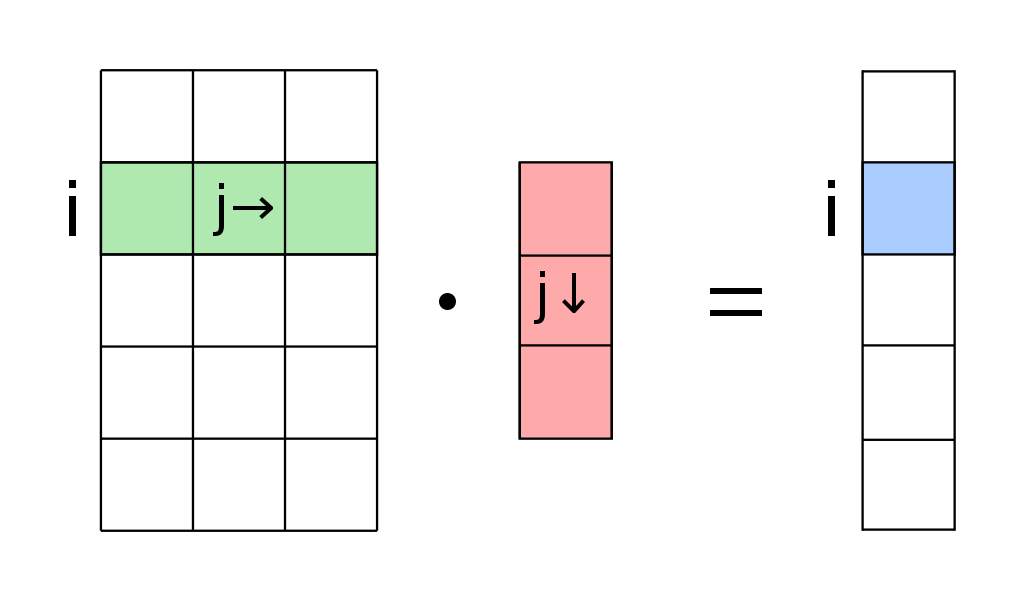
\includegraphics[width=\textwidth, height=\textheight, keepaspectratio]{chapters/chapter 2/mvm.png}
\end{marginfigure}\[
  A\mathbf{v} = \begin{bmatrix}
    a_{11}v_1 + a_{12}v_2 + \ldots + a_{1n}v_n \\
    a_{21}v_1 + a_{22}v_2 + \ldots + a_{2n}v_n \\
    \vdots \\
    a_{m1}v_1 + a_{m2}v_2 + \ldots + a_{mn}v_n \\
  \end{bmatrix}
\]
Արդյունքում ստացված $m$-չափանի վեկտորը կոչվում է \textbf{$A$ մատրիցի և $\vv$ վեկտորի արտադրյալ։} 
\end{definition}

Այլ կերպ ասած՝ եթե $A$-ի տողերը նշանակենք $\mathbf{A}_1, \mathbf{A}_2, \ldots, \mathbf{A}_m$՝\marginnote{\bigskip \bigskip \bigskip \bigskip $\mathbf{A}_i$-երը կլինեն $n$-չափանի վեկտորներ}
\[
A = \begin{bmatrix}
\dots& \mathbf{A}_1 & \ldots \\
\dots& \mathbf{A}_2 & \ldots \\
 & \vdots &  \\
\dots& \mathbf{A}_m & \ldots \\
\end{bmatrix}
\]
ապա 
\begin{itemize}
\item $A\vv$-ի առաջին բաղադրիչը կլինի $\mathbf{A}_1 \cdot \vv$ սկալյար արտադրյալը,
\item $A\vv$-ի երկրորդ բաղադրիչը կլինի $\mathbf{A}_2 \cdot \vv$ սկալյար արտադրյալը,
\end{itemize}
և այդպես շարունակ՝
\[
A\mathbf{v} = \begin{bmatrix}
a_{11}v_1 + a_{12}v_2 + \ldots + a_{1n}v_n \\
a_{21}v_1 + a_{22}v_2 + \ldots + a_{2n}v_n \\
\vdots \\
a_{m1}v_1 + a_{m2}v_2 + \ldots + a_{mn}v_n \\
\end{bmatrix}= \begin{bmatrix}
\mathbf{A}_1 \cdot \mathbf{v} \\
\mathbf{A}_2 \cdot \mathbf{v} \\
\vdots \\
\mathbf{A}_m \cdot \mathbf{v} \\
\end{bmatrix} 
\]

\begin{example}
\[
  A = \begin{bmatrix}
    1 & 2 & 3 \\
    4 & 5 & 6 \\
  \end{bmatrix}
  \qquad
  \mathbf{v} = \begin{bmatrix}
    2 \\
    -1 \\
    3 \\
  \end{bmatrix}
\]
\[
  A\mathbf{v} = \begin{bmatrix}
    1 \cdot 2 + 2 \cdot (-1) + 3 \cdot 3 \\
    4 \cdot 2 + 5 \cdot (-1) + 6 \cdot 3 \\
  \end{bmatrix}
  = \begin{bmatrix}
    9 \\
    21 \\
  \end{bmatrix}
\]
\end{example}

Ինչ-որ իմաստով՝ մատրիցի ու վեկտորի բազմապատկումը մեր իմացած սկալյար արտադրյալի ընդհանրացումն է։ Ի սկզբանե գիտեինք, թե ինչպես բազմապատկել վեկտորը վեկտորով։ Իսկ մատրիցը ոչ այլ ինչ է, քան իրար տակ գրված մի քանի վեկտոր։ Ինչպե՞ս պիտի բազմապատկեինք այդ «մի քանի վեկտորը» մեկ այլ $\vv$ վեկտորի հետ․ բնական կլիներ հերթով դրանցից յուրաքանչյուրը բազմապատկել $\vv$-ով, ապա ստացվածները գրել իրար տակ (ինչը և արեցինք)։

\begin{example}
\[
  A = \begin{bmatrix}
    -2 & 1 \\
    0 & 3 \\
    1 & -1 \\
  \end{bmatrix}
  \qquad
  \mathbf{v} = \begin{bmatrix}
    4 \\
    2 \\
  \end{bmatrix}
\]
\[
  A\mathbf{v} = \begin{bmatrix}
    (-2) \cdot 4 + 1 \cdot 2 \\
    0 \cdot 4 + 3 \cdot 2 \\
    1 \cdot 4 + (-1) \cdot 2 \\
  \end{bmatrix}
  = \begin{bmatrix}
    -6 \\
    6 \\
    2 \\
  \end{bmatrix}
\]
\end{example}


Այնուամենայնիվ, ինչո՞ւ պետք է ուզենք վեկտորը բազմապատկել մատրիցով։
Մտովի պատկերեք տարածության մեջ մի քանի վեկտոր՝ որպես սլաքներ։\marginnote{\href{https://visualize-it.github.io/linear_transformations/simulation.html}{այստեղ} սեղմելով {\rm transform}՝ կտես\-նեք, թե ինչ է տեղի ունենում վեկ\-տորները բեր\-ված մատրիցով բազմապատկելիս}
Ինչպես կտեսնենք հաջորդ թեմայում, վեկտորները մատրիցով բազմապատկելը երկրաչափորեն նույնն է, ինչ այդ վեկտոր\-ները ինչ-որ մի անկյան տակ պտտելը, և դրանց ինչ-որ ուղղությամբ սեղմելը կամ ձգելը։ Այլ կերպ ասած՝ երբ վեկտորները բազմապատկում ենք մատրիցով, դրանք \textit{ձևափոխվում} են։ 

Ընդ որում՝ այդ ձևափոխությունը տեղի ունենալու ժամանակ պահպան\-վում են հետևյալ կանոնները՝
\begin{enumerate}
    \item $A(\vv+\vu)=A\vv + A\vu$
    \item $A(c \cdot \vv) = c \cdot A\vv$
\end{enumerate}
այսինքն՝ 
\begin{enumerate}
    \item ձևափոխել, հետո գումարել $=$ գումարել, հետո ձևափոխել
    \item ձգել, հետո ձևափոխել $=$ ձևափոխել, հետո ձգել
\end{enumerate}

Այս հատկությունների շնորհիվ մատրիցով բազմապատկման գործո\-ղու\-թյունը կանվանենք նաև \textit{գծային ձևափոխություն,} և կասենք՝ $A$ մատրիցը/գծային ձևափոխությունը \textbf{կիրառել} $\vv$ վեկտորի վրա։ Այս մասին ավելի մանրամասն կխոսենք հաջորդ թեմայում։

\question{Ի՞նչ մատրից կիրառենք $[4 \quad 5]$ վեկտորի վրա, որպեսզի այն երկու անգամ ձգվի։}



\section{Մատրիցների բազմապատկումը}

Եվ իհարկե, սահմանենք երկու մատրիցների արտադրյալը՝ մոտա\-վո\-րա\-պես նույն տրամաբանությամբ։

\begin{definition}\label{mmm}
Ենթադրենք $A$-ն \(m \times n\) մատրից է, իսկ $B$-ն՝ $n \times k$ մատրից։\marginnote{$A$-ի սյուների թիվ $=$ $B$-ի տողերի թիվ} $A$ և $B$ \textbf{մատրիցների արտադրյալը} կլինի $m \times k$ չափանի մատրից, որի $i$-րդ տողի $j$-րդ տարրը հավասար է $A$-ի $i$-րդ տողի և $B$-ի $j$-րդ սյան սկալյար արտադրյալին։
\[
A = \begin{bmatrix}
a_{11} & a_{12} & \ldots & a_{1n} \\
a_{21} & a_{22} & \ldots & a_{2n} \\
\dots & \dots & \dots & \dots \\        a_{m1} & a_{m2} & \ldots & a_{mn} \\
\end{bmatrix}
\qquad
B = \begin{bmatrix}
b_{11} & b_{12} & \ldots & b_{1k} \\
b_{21} & b_{22} & \ldots & b_{2k} \\
\dots & \dots & \dots & \dots \\        b_{n1} & b_{n2} & \ldots & b_{nk} \\
\end{bmatrix}
\]\begin{marginfigure}    
\includegraphics[width=\textwidth, height=\textheight, keepaspectratio]{chapters/chapter 2/mmm.png}
\end{marginfigure}\[
AB = \begin{bmatrix}
c_{11} & c_{12} & \ldots & c_{1k} \\
c_{21} & c_{22} & \ldots & c_{2k} \\
\dots & \dots & \dots & \dots \\
c_{m1} & c_{m2} & \ldots & c_{mk} \\
\end{bmatrix}
\]
որտեղ $\displaystyle c_{ij} = a_{i1}b_{1j} + a_{i2}b_{2j} + \ldots + a_{in}b_{nj}= \sum_{p=1}^{n} a_{ip}b_{pj}$:
\end{definition}

Այսինքն՝ ձախ մատրիցի ամեն մի տողը բազմապատկում ենք (սկալյա\-րա\-պես) աջ մատրիցի ամեն մի սյան հետ։

\begin{example}
\[
  C = \begin{bmatrix}
    -1 & 0 \\
    2 & -3 \\
    4 & 1 \\
  \end{bmatrix}\in \R^{3 \times 2}
  \qquad
  D = \begin{bmatrix}
    5 & -2 & 1 \\
    3 & 0 & 7 \\
  \end{bmatrix}\in \R^{2 \times 3}
\]
\begin{align*}
  CD &= \begin{bmatrix}
    -1 \cdot 5 + 0 \cdot 3 & -1 \cdot (-2) + 0 \cdot 0 & -1 \cdot 1 + 0 \cdot 7 \\
    2 \cdot 5 + (-3) \cdot 3 & 2 \cdot (-2) + (-3) \cdot 0 & 2 \cdot 1 + (-3) \cdot 7 \\
    4 \cdot 5 + 1 \cdot 3 & 4 \cdot (-2) + 1 \cdot 0 & 4 \cdot 1 + 1 \cdot 7 \\
  \end{bmatrix}
 \\&= \begin{bmatrix}
    -5 & 2 & -1 \\
    1 & -4 & -19 \\
    23 & -8 & 11 \\
  \end{bmatrix}\in\R^{3 \times 3}
\end{align*}
\end{example}

\question{Ի՞նչ կստացվեր, եթե վերևի օրինակում բազմապատկեինք այսպես՝ $DC$։}


\warning{Երկու մատրից հնարավոր է բազմապատկել միայն եթե առաջին մատրիցի սյուների թիվը (այսինքն՝ դրա տողերի երկարությունը) համընկնում են երկրորդի տողերի թվի (սյուների երկարության) հետ։}

Հետևաբար ոչ բոլոր մատրիցներն է հնարավոր իրարով բազմապատկել։

\question{Հնարավո՞ր է, որ երկու $A$, $B$ մատրից կարելի լինի բազ\-մա\-պատկել այսպես՝ $AB$, բայց ոչ այսպես՝ $BA$:}

Եթե չիմանայինք վեկտորների սկալյար արտադրյալի մասին, շատ տարօրինակ կլիներ մատրիցների արտադրյալը այս ձևով սահմանելը (իրոք, կարող էինք պարզապես բազմապատկումը սահմանել ասենք՝ տարր առ տարր)։ 

Իսկ այսպես սահմանելու դեպքում, եթե փորձեք օրինակ՝ ինչ-որ $A$ մատրից բազմապատկել $\vv$ վեկտորով, անկախ նրանից՝ $\vv$-ն կհամարեք վեկտոր \marginnote{նկատենք, որ $\va \cdot \vb = \va^T \vb$} և կօգտվեք \hyperref[mvm]{\color{OliveGreen} սահմանում \ref*{mvm}}-ից, թե կհամարեք այն $1$ սյունից բաղկացած մատրից ու կօգտվեք \hyperref[mmm]{\color{OliveGreen} սահմանում \ref*{mmm}}-ից, երկու դեպքում էլ կստանաք նույնը։

Նկատենք նաև, որ ինչպես բոլոր նախորդ գործողություններում, մատրիցների բազմապատկումը նույնպես օժտված է հետևյալ լավ հատկություններով՝
\begin{itemize}
\item $A(B + C) = AB + AC$ և  $(A + B)C = AC + BC$\marginnote{փակագծերը կարող ենք բացել}

\item $A(BC) = (AB)C$ \marginnote{կարևոր չէ՝ սկզբից $BC$-ն, թե $AB$-ն}

\item $A(cB) = c(AB)=(cA)B$\marginnote{ցանկացած $c\in\R$ թվի համար}
\end{itemize}



\bigskip 

\begin{theory}
.
\begin{itemize}
\item կարդալ [{\rm Johnston}], 121-124 (գծային տարածություններ), 35-38 (գծային ձևափոխություններ) էջերը
\item կարդալ [{\rm Poole}], 219-221 էջերը (մատրիցների արտադրյալ)
\item դիտել  {\rm 3b1b}-ի \href{https://www.3blue1brown.com/lessons/linear-transformations}{3-րդ տեսադասը} գծային հանրահաշվից \end{itemize}
\end{theory}

\newpage

\section{Խնդիրներ}

\begin{problem}\marginnote[*+0.5]{\href{https://youtu.be/N8GR7eCepl8}{նման խնդրի լուծում}}
Արդյո՞ք տրված բազմությունը գծային տարածություն է․

\begin{enumerate}[label={\alph*}․]
\item $A = \bigg\{ \begin{bmatrix} a \\ 0 \end{bmatrix} \mid \text{ բոլոր }a\in\R \text{ թվերի համար} \bigg\}$

\item \marginnote{\medskip $\R^2$ հարթության ո՞ր ուղիղն է սա}$B = \bigg\{ \begin{bmatrix} a \\ -a \end{bmatrix} \mid  \text{բոլոր }a\in\R \text{ թվերի համար} \bigg\}$

\item $C =  \bigg\{ \begin{bmatrix} a \\ 1 \end{bmatrix} \mid \text{ բոլոր }a\in\R \text{ թվերի համար}\bigg\}$

\item $D = \mathbb{Z}$ ամբողջ թվերի բազմությունը

\item $ax+b$ տեսքի բոլոր բազմանդամների բազմությունը

\item $ax+b$ տեսքի այն բազմանդամների բազմությունը, որոնցում $a \ne 0$
\end{enumerate}
\end{problem}


\hint{Եթե ցույց տանք, որ 1-9 պայմաններից գոնե մեկը խախտվում է, ապա բազմությունը գծային տարածություն չէ։ Եթե բոլոր 1-9 պայմանները միշտ տեղի ունեն, ապա բազմությունը գծային տարածություն է։}


\begin{problem}
Ի՞նչ կստանանք
\[
A = \begin{bmatrix}
    3 & -3 \\
    3 & 3
\end{bmatrix}
\] 
մատրիցը կիրառելով հետևյալ վեկտորների վրա․
\begin{enumerate}[label={\alph*}․]
\item $\va=\begin{bmatrix}
    1 \\ 0
\end{bmatrix}$

\item $\vb=\begin{bmatrix}
    0 \\ 1
\end{bmatrix}$

\item $\vc=\begin{bmatrix}
    1 \\ 1
\end{bmatrix}$
\end{enumerate}

Կոորդինատային հարթության վրա պատկերեք վեկտորներից յուրաքան\-չ\-յու\-րը մինչև $A$-ով բազմապատկելը և դրանից հետո։ Ի՞նչ եք տեսնում, ի՞նչ է անում մատրիցը վեկտորների հետ։ Կարո՞ղ եք գուշակել, թե ինչպես կձևափոխվի $\begin{bmatrix}
    2 & -2
\end{bmatrix}$ վեկտորը։
\end{problem}

\begin{problem}
Հաշվեք մատրիցների արտադրյալը․
\begin{enumerate}[label={\alph*}․]
\item $AB$, որտեղ $A=\begin{bmatrix}
6&5\\-2&7  \end{bmatrix}$, $B=\begin{bmatrix}
-5&3\\1&4   \end{bmatrix}$

\item $(A-B)(A+B)$, որտեղ $A=\begin{bmatrix}
2&2&4\\-3&-2&4\\-2&0&2   \end{bmatrix}$, $B=\begin{bmatrix}
2&1&3\\-1&2&2\\1&4&-1   \end{bmatrix}$

\item $A^2 - B^2$, նույն $A$ ու $B$-ով, ինչ \textit{բ․}-ում
\end{enumerate}

Նո՞ւյնն են արդյոք \textit{բ․}-ում ու \textit{գ․}-ում ստացված մատրիցները։
\end{problem}

\begin{problem}
Դիտարկենք հետևյալ մատրիցը (կոչվում է \textit{շեղման} կամ \textit{սահքի մատրից})՝\marginnote{անգլերեն՝ {\it shear matrix}}
\[
S = \begin{bmatrix}
    1 & 1 \\ 0 & 1
\end{bmatrix}
\]
\begin{enumerate}[label={\alph*}․]
\item ի՞նչ կստանանք, եթե $S$-ը կիրառենք $\begin{bmatrix}
    0 & 1
\end{bmatrix}$ վեկտորի վրա

\item ի՞նչ կստանանք, եթե $S$-ը կիրառենք ստացված վեկտորի վրա

\item ի՞նչ կստանանք, եթե մի անգամ էլ կիրառենք $S$-ը

\item ի՞նչ եք կարծում, ի՞նչ կստանանք, եթե $S$-ը կիրառենք $100$ անգամ այդ վեկտորի վրա

\item կարո՞ղ եք հաշվել $S^{100}$-ը
\end{enumerate}
\end{problem}


\begin{problem}\marginnote{\bigskip \href{https://youtu.be/fM2H49xwXS8}{լուծում}}
Ենթադրենք $A$-ն այնպիսի մատրից է, որ
\[
A\begin{bmatrix}
    1 \\ 2
\end{bmatrix}
=
\begin{bmatrix}
    -3 \\ 5
\end{bmatrix},
\qquad 
A\begin{bmatrix}
    3 \\ 5
\end{bmatrix}
=
\begin{bmatrix}
    7 \\ 1
\end{bmatrix}
\]
Քանի՞սը քանիսի վրա է $A$ մատրիցը։ Գտեք $A$-ն։
\end{problem}









% \begin{problem}
% Տրված են հետևյալ վեկտորները՝
% \[
% \va= \begin{bmatrix} 3 \\ -1 \\ 2 \end{bmatrix}, \qquad \vb=\begin{bmatrix} 2 \\ 4 \\ -5 \end{bmatrix}, \qquad \vc = \begin{bmatrix}
%     5 \\ 6.5 \\ -7
% \end{bmatrix}
% \]

% Գտեք արտահայտության արժեքը․
% \begin{enumerate}[label={\alph*}․]
% \item $\va+\vb$
% \item $\va+\vb-\vc$
% \item $\va^T+\vb^T-\vc^T$
% \item $3\va^T+4\vb^T-2\vc^T$
% \item $6\va^T+8\vb^T-4\vc^T$
% \item $\va \cdot \vb$
% \item $(3\va - 6\vb) \cdot \vc$
% \item $\va \cdot (4\va^T - \vb^T)^T$
% \end{enumerate}
% \end{problem}

% \begin{problem}
% Թարգմանչական գրասենյակը թարգմանեց  $\va=\begin{bmatrix}
%     24 & 17 & 9 & 13
% \end{bmatrix}$ փաստաթուղթ համապատասխանաբար անգլերեն, ֆրանսերեն, գերմաներեն և ռուսերեն։ Յուրաքանչյուր լեզվի համար մեկ էջ թարգմանելը տևում է մոտավորապես $\vb=\begin{bmatrix}
%     5 & 10 & 11 & 7
% \end{bmatrix}$ րոպե։ 

% \smallskip

% Ընդհանուր որքա՞ն ժամանակ պահանջվեց փաստաթղթերը թարգմանելու համար։ Միջինում քանի՞ րոպե ծախսեց թարգմանիչներից յուրաքանչյուրը, եթե գրասենյակում կա $4$ թարգմանիչ։ Պատասխանը արտահայտեք $\va$-ով և $\vb$-ով։
% \end{problem}

% \begin{problem}
% Հաշվեք հետևյալ վեկտորների մանհեթընյան և էվկլիդյան նորմերը․

% \begin{enumerate}[label={\alph*}․]
% \item $\va= \begin{bmatrix} 2\\-9\\3 \end{bmatrix}$

% \item $\va-2\vb$, որտեղ $\va= \begin{bmatrix}3\\4\\1\\0\end{bmatrix},\  \vb = \begin{bmatrix}4\\5\\-2\\-1\end{bmatrix}$

% \item $-3\vc$, որտեղ $\vc= \begin{bmatrix}2\\-5\\6\end{bmatrix}$
% \end{enumerate}
% \end{problem}

% \begin{problem}
% Որքա՞ն անկյուն են կազմում
% \begin{enumerate}[label={\alph*}․]
% \item $\va= \begin{bmatrix} 2\\1\\1\end{bmatrix}$ և $\vb= \begin{bmatrix} 1\\-3\\3\end{bmatrix}$ վեկտորները

% \item նախորդ խնդրի $\va$ ու $\vc$ վեկտորները
% \end{enumerate}
% \end{problem}


% \begin{problem}
% Ամենաշատը քանի՞ վեկտոր կարող ենք տեղադրել $\R^2$ հարթության մեջ, որպեսզի ցանկացած երկուսի սկալյար արտադրյալը լինի դրական։ Իսկ որպեսզի լինի բացասակա՞ն։
% \end{problem}
